% !TeX spellcheck = en_GB
\documentclass[11pt,fleqn]{article}

\usepackage[english]{babel}
\usepackage{SpeedyGonzales}
\usepackage{MediocreMike}
%\usepackage{Blastoise}
\usepackage{float}
\usepackage[caption = false]{subfig}

\title{Course 02445 -- Project II\\Phosphate in Soil and the Effect on Barley Production}
\author{Asger Laurits Schultz and Søren Winkel Holm\\s183912 and s183911}
\date{\today}

\fancypagestyle{plain}
{
	\fancyhf{}
	\rfoot{Page \thepage{} af \pageref{LastPage}}
	\renewcommand{\headrulewidth}{0pt}
}
\pagestyle{fancy}
\fancyhf{}
\lhead{Asger Laurits Schultz\\Søren Winkel Holm}
\chead{\today}
\rhead{Course 02445\\Project II}
\rfoot{Page \thepage{} af \pageref{LastPage}}

\graphicspath{{Billeder/}}
\linespread{1.15}
\usepackage{hyperref}

%\numberwithin{equation}{section}
%\numberwithin{footnote}{section}
%\numberwithin{figure}{section}
%\numberwithin{table}{section}

\begin{document}

\maketitle
%\thispagestyle{fancy}
%\tableofcontents
%-- Compare measurement methods of bioavailable phosphorous and examine the influence of bioavailable phosphorous on harvest yield. 
%-- By the explanatory strengths of the two measurements, the DGT measurement is found to be most useful in predicting the yield.
%-- Bioavailable phosphorous is using both measurements found to have significant effect on the yield \(p<10^{-9}\).
\tableofcontents

\newpage
\begin{abstract}
	Farm yields depend on a large variety of factors including phosphate concentrations in the soil. Using data from nine fields in Denmark and Norway, we attempt to answer two questions: Is there a statistically significant difference between the predictive abilities of data from different measurement methods (Olsen P and DGT), and does the amount of bioavailable phosphorus impact the yield? We use both linear models and the Michaelis-Menten model are used to model the yield as a function of the phosphate availability, and their errors are compared using $ t $ test. We use ANCOVA to test for a significant impact on harvest yield. We find that the DGT measurements have more explanatory power, though not enough to be statisticallly significant ($ p=0.21 $). The ANCOVA shows that the amount of phosphate impacts the harvest yields ($ p=2\ctp{-10} $ for Olsen P and $ p=4\ctp{-13} $ for DGT), though the model assumptions are only somewhat fulfilled.
\end{abstract}

\section{Introduction}
A wide range of very different effects are in play in determining the output yield of a farm.
As environmental and economic incentives rise, there is increasing motivation for precision agriculture which optimizes the performance of farming using ecological, chemical and biological variables.
One of these important variables is the nutrient of the soil and \textit{phosphorous} is essential in this regard.


This report considers different techniques for measuring the amount of phosphorous available to the plants and compares two measurement methods, the traditional "Olsen-P" and the newer "DGT" method, using the output yield of barley fields as the target.  
Correlations, model fitting of Michaelis-Menten models and ANCOVA models are used to examine the connections between the measurements and the yield output.

All code is available in the \texttt{src} folder at \url{https://github.com/sorenmulli/02445projects.git}.

\section{Data}
The data consists of 100 observations each consisting continuous  Olsen-P measurements [mg/100g], DGT-measurements [\(\mu\)g/L] and harvest yield of barley [hkg/ha] and categorical location id's for the field on which the observations were made. Nine fields have been surveyed and given id's from "001" to "011". The last field has missing values for two of it's three yield measurements.  

The fields are from Denmark and Norway and the multiple measurements of yield from each field correspond to division of the fields into plots from which soil samples were taken and later barley output was recorded such that these measurements cannot be considered independent which is visualized in figure \ref{fig:fieldbox}. Further visualization of the data is given in the results section where scatter plots are supplied.
\begin{figure}[H]
	\centering
	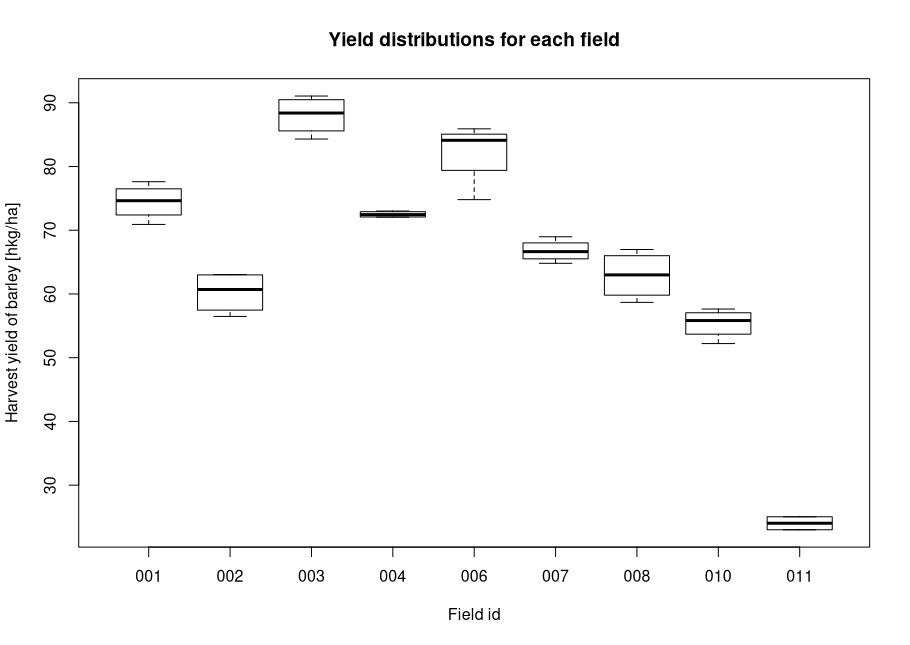
\includegraphics[width=.7\linewidth]{p2_fieldbox}
	\caption{Boxplot of the barley output measurements for the plots in each field. Note the much larger between-field variance than within-field variance which shows that the multiple observations on the same field cannot be considered independent.}
	\label{fig:fieldbox}
\end{figure}
\section{Methods and analysis}
\subsection{Recommended measure}
Without access to a verifiable measurement of bioavailable phosphorous, the measurement methods are evaluated based on their ability to explain, and thus, predict the yield of the field. 

As an initial examination, the correlation between yield output and each phosphorous measurement is found and visualized to account for linear relationships. The correlation between the two measurements is also included together with visualizations of the significance of the correlations.

To test which measurement predicts the barley yield best beyond linear tendencies, Michaelis-Menten models are used. The nonlinear model is connected to the reaction velocity of enzymes such as nutrients \cite{michment} and assumes that:
\[
y = \frac{\alpha x}{\beta + x}, x >0
\]
This nonlinear model is fitted using the yield as target variable and both DGT measurements and Olsen P-measurements as explanatory variables by the R function \texttt{nls} which iteratively fits the parameters using a squared loss criterion.  To estimate the generalization error of each model, leave-one-out cross-validation over the fields is performed by fitting the models to eight out of the nine and evaluating them on the last for all fields. The starting guesses for each model is kept constant.

From this, estimates of the two model's generalization errors as the mean squared error loss are found and these are compared with a $t$ test on test errors of the nine folds to evaluate the evidence for the hypothesis that modelling using one measurement technique is better than using the other.
\subsection{Yield influence of bioavailable phosphorous}
To test whether there is a significant effect of bioavailable phosphorous on the barley yield, ANCOVA models of the following form is evaluated:
\[
y_i = \alpha_{field(y_i)} + \beta x_i + \epsilon_i, \quad \epsilon_i \sim \mathcal N (0, \sigma^2)
\]
where \(y\) is the barley yield and two models are evalued with \(x\) being the DGT and the Olsen-P measurements respectively. Interaction effects are not included due to the missing data in one of the fields such that only one slope is evaluated for each model. The significance of this slope -- and thus the linear effect of bioavailable phosphorous -- is then evaluated using the ANCOVA F-test for each model.
\section{Results}
\begin{figure}[H]
	\centering
	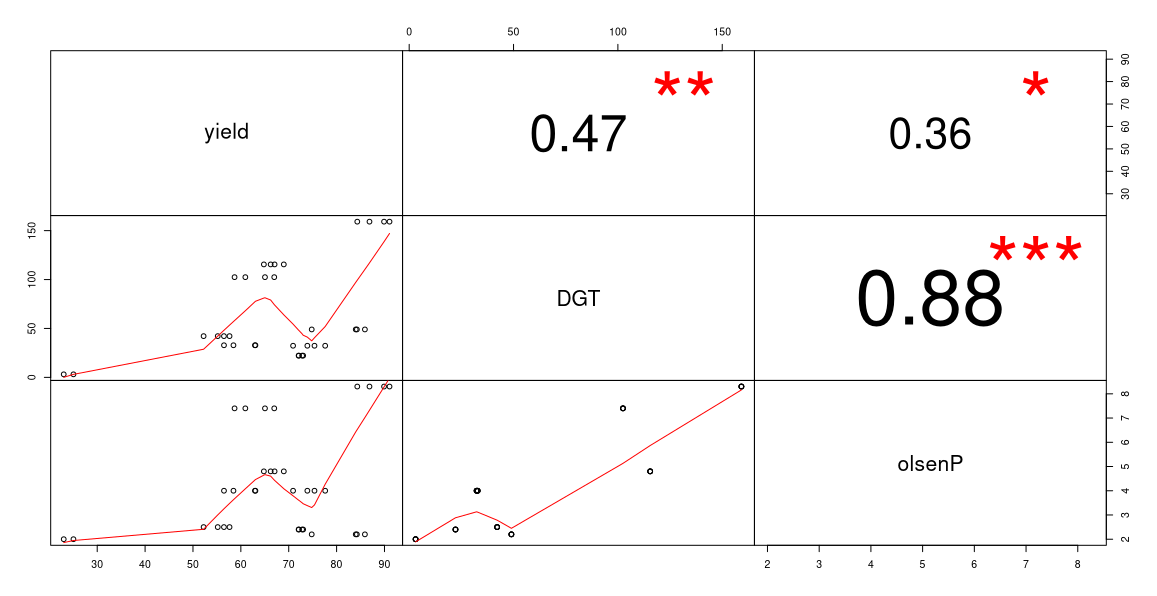
\includegraphics[width=.75\linewidth]{p2_corrplot}
	\caption{Scatter plots with rolling averages and correlations between the three continous variables. Asterisks are loose indications\protect\footnotemark\ of amount of evidence for the hypothesis that the correlation \(\neq 0\).}
\end{figure}
\footnotetext{They are computed with \texttt{corr.test} but the assumptions for these to count as \(p\) values (where one asterisk corresponds to \(\alpha = 0.05\) and so forth) are not fulfilled as the data points are not independent}
\begin{figure}[H]
	\centering
\subfloat{
	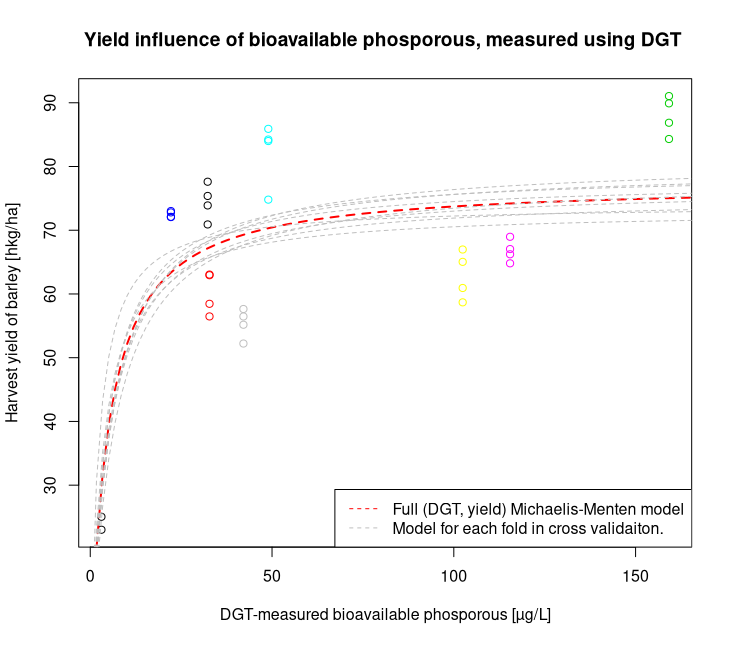
\includegraphics[width=.5\linewidth]{dgt_mmm}
}
\subfloat{
	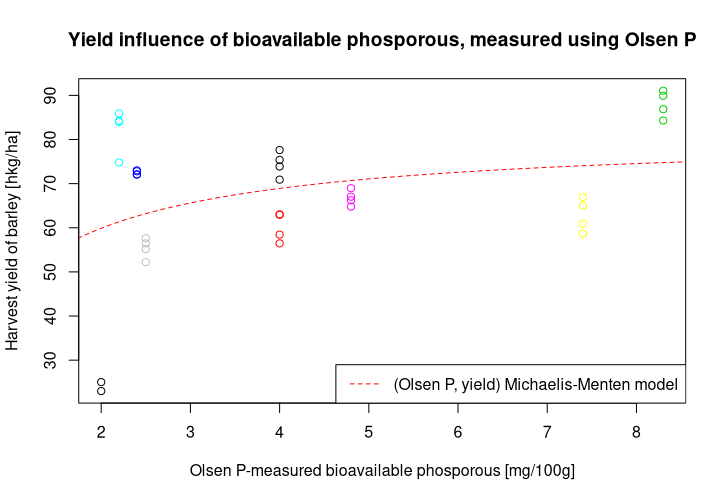
\includegraphics[width=.5\linewidth]{oP_mm}
}	
	\label{fig:yield_bio}
\caption{Michaelis-Menten models with visualizations of the nine cross validation folds.}
\end{figure}
The estimated generalization errors from the nine-fold cross validation over the fields:
\begin{align*}
	& \widehat {MSE}_{gen} ^{dgt} = 181
	&& \widehat {MSE}_{gen} ^{olsenP} = 445
\end{align*}
The paired \(t\) test comparison of the nine cross validation test errors for the two models including 95\pro\ confidence interval and \(p\) value for \(H_0: {MSE}_{gen} ^{dgt}={MSE}_{gen} ^{olsenP}\):
\[
\widehat{\Delta MSE}_{gen} = -264, \quad \Delta MSE\in [-713, 185],\quad  p=0.21
\]
%\begin{figure}[H]
%	\centering
%	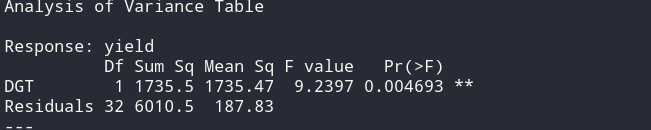
\includegraphics[width=.7\linewidth]{simpleDGT}
%\end{figure}



%\begin{figure}[H]
%	\centering
%	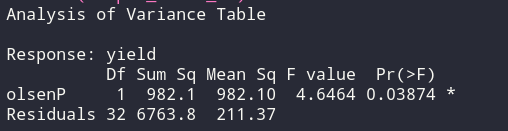
\includegraphics[width=.7\linewidth]{simpleOP}
%\end{figure}
\noindent
The results of the ANCOVA and corresponding \(F\)-test:  
\begin{table}[H]
	\centering
	\begin{tabular}{c | c c c c}
	\textbf{DGT-model}  &Degrees of freedom & MSE&\(F\)-value&\(p\)-value\\
	\hline 
	Location  & 1& 826 & 90 & \(4\ctp{-16}\)\\
	DGT  & 7&1735 &  188 & \(4\ctp{-13}\)\\
	Residuals &25 &9.23 &\\
	\hline 
	\textbf{Olsen P-model} &Degrees of freedom & MSE&\(F\)-value&\(p\)-value\\
	\hline 
	Location & 1&933 & 101 & \(<2.2\ctp{-16}\)\\
	Olsen P &7 &982 & 106 & \(2 \ctp{-10}\)\\
	Residuals &25  &9.23
	\end{tabular}
\end{table}\noindent 
The slopes for the ANCOVA models and their std. errors are estimated to:
\begin{align*}
	&\hat \beta_{dgt}= 1.7,\ \ \hat \sigma_{\beta_{dgt}}=0.090
	&&\hat \beta_{olsenP}= 25,\ \ \hat \sigma_{\beta_{dgt}}=1.3
\end{align*}
\section{Discussion}
\paragraph{Validity of statistical analyses} The assumptions of \(t\) test of independence and normality are considered as partly satisfied as the experiment setup is assumed to supply independence between the fields but the normality of the paired test is somewhat more doubtful with the outliers shown in the quantile-quantile on figure \ref{fig:qq}. Also, with only nine data points used for the test, the $ t $ test should by no means be taken as an absolute truth.
\begin{figure}[H]
	\centering
	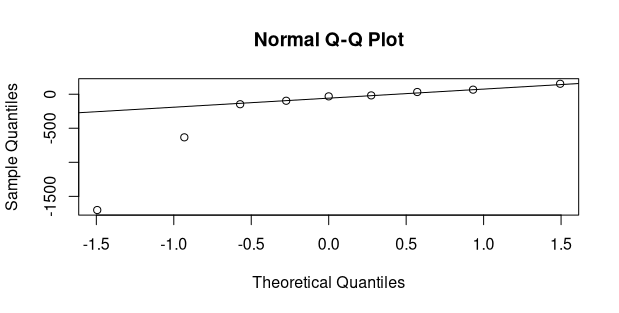
\includegraphics[width=.5\linewidth]{p2_t_qq}
	\label{fig:tqq}
	\caption{Quantiles/quantile plot of the differences in \(MSE\) used to check for normality of the the paired $t$ test. Two left-skewing outliers problematize the normal assumption.}\label{fig:qq}
\end{figure} \noindent 
For the ANCOVA, the assumption of linears effects is doubtful as the Michaelis-Menten nonlinear model fits better to the data than linear models. The assumption of variance homogeneity can neither be confirmed with some of the fields having lower variance though this beyond conclusion with just 2-4 data points for each field. The normality assumption seems reasonable based on below plots bar some askewness.
\begin{figure}[H]
	\centering
	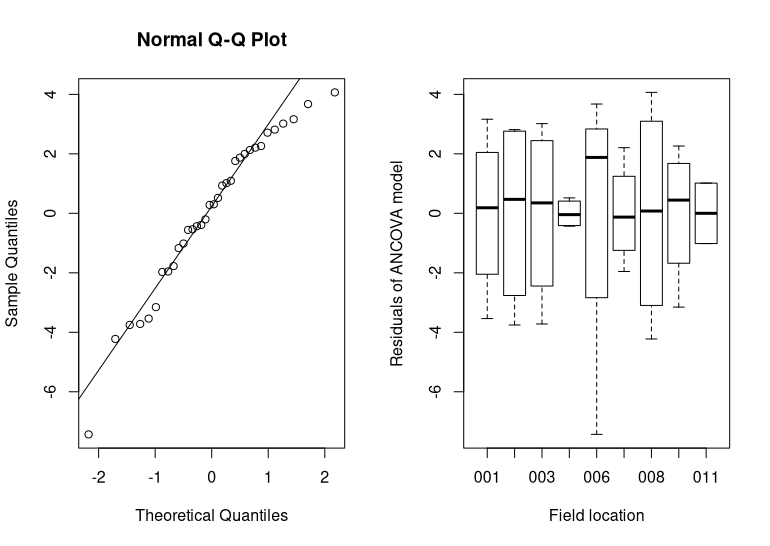
\includegraphics[width=.75\linewidth]{p2_ancova_qq}
	\label{fig:tqq}
	\caption{Quantiles/quantile plot of ANCOVA residuals and boxplot of field group residuals. Note that these plots are the same for both ANCOVA models as the only one DGT and one Olsen P measurement has been made for each field.}
\end{figure} \noindent 
\paragraph{Statistical conclusions} The estimates of the generalization errors of the Michaelis-Menten models implied a clear edge of the DGT measurement in terms of explanatory power. 
However, due to the \(t\)-test returning \(p=0.21\) and not being completely validated, the statistical evidence for this edge to be significant is minor or non-existant. This could be further tested with a non-parametric rank-sum test but it is suspected that no significant evidence can be found of this difference without more data.

The ANCOVA proves more convincingly the simple fact that both measurements have significant effects on the barley yield with very low \(p\)-values. 
Though they cannot be interpreted directly as risk of type I-errors due to limited fulfilment of assumptions, the \(p\)-values are seen as high degree of evidence for the effect of the bioavailable phosphorous.

\paragraph{Recommendations} The first, clear recommendation is that no matter what measurement technique the farmers use, the amount of bioavailable phosphorous is linked to yield of barley. 
This is supported by the ANCOVA conclusions, the correlations of 0.36 and 0.46 and the Michaelis-Menten models' explanatory power which is considered as an approximation of the true enzymological, generative story \cite{michment}. 
This of course, does not prove that the bioavailable phoshorous \textit{causes} the higher yield, though this is suspected due to the role of phosphorous in nutrients and the Michaelis-Menten model is recommended as a possible model for this effect which can help farmers plan the crop rotation and choice of farming land.

It was ultimately not proven that the newer DGT measurement predicts the yield better than the cheaper Olsen P-measurement but a number of indicia were found which give some evidence for this: The DGT measurement had the highest correlation with the yield, the DGT Michaelis-Menten model fitted better to the data and the DGT measurement explained a higher amount of the variance in the ANCOVA models than the Olsen-P measurement did.
Based on this, collection of more data is suggested and it is recommended for farmers to use the DGT measurement if the economic loss of this is minor. 

On the other hand, the correlation between the measurement techniques was found to be 88\pro\ so a major investment in the new technique cannot be justified based on this evidence. 
An important factor in the hinted, higher predictive power of the DGT measurement was field 11 which had the lowest yield and can be seen as the outlier in the figures \ref{fig:fieldbox}, \ref{fig:tqq} and in figure \ref{fig:yield_bio} it is clear that the model based on DGT-measurements explains this field (points in light grey) much better. 
If the data corresponds well to the general field distribution and the Michealis-Menten model is a good approximation of the generative story, a heuristic can be formed that the DGT-technique should be used on low-yield fields. 
On the other hand, if field 11 is seen as an outlier which should be excluded from the models (an idea somewhat supported by the two NA's in the four yield measurements from field 11), then the evidence for the advantage of DGT shrinks considerably.


\begin{thebibliography}{9}
	\bibitem{michment}Dragan, J., Kristian, S., Scitovski, R.: "Total least squares fitting Michaelis–Menten enzyme kinetic model function", 04-07, Journal of Computational and Applied Mathematics, 201:1. 

\end{thebibliography}
\end{document}

















